\documentclass[UTF8,a4paper,10pt,twoside]{ctexbook}



\usepackage{fancyhdr}

\usepackage[
  portrait,
  marginparwidth=126pt,
  marginparsep=5pt,
  textwidth = 385pt,
  textheight = 618pt,
  includehead=false,
  includefoot=false,
  ignoremp=false,
  includemp
]{geometry}



\pagestyle{fancy}
% with this we ensure that the chapter and section
% headings are in lowercase.
\renewcommand{\chaptermark}[1]{\markboth{#1}{}}
\renewcommand{\sectionmark}[1]{\markright{\thesection\ #1}}
\fancyhf{} % delete current setting for header and footer
\fancyhfoffset[LE,RO]{131pt}
\fancyfoot[LE,RO]{\bfseries\thepage}
\fancyhead[LE]{\bfseries\rightmark}
\fancyhead[RO]{\bfseries\leftmark}
\renewcommand{\headrulewidth}{0.5pt}
\renewcommand{\footrulewidth}{0pt}
\addtolength{\headheight}{0.5pt} % make space for the rule
\fancypagestyle{plain}{%
\fancyhead{} % get rid of headers on plain pages
\renewcommand{\headrulewidth}{0pt} % and the line
}






\usepackage{amsmath}
\usepackage{float}
\usepackage{tikz}
\usetikzlibrary{shapes,arrows,arrows.meta,positioning,calc,shadows,graphs}

\usepackage[colorlinks = true,linkcolor=black]{hyperref}


\usepackage{multicol}
\usepackage{multirow}









\title{计算机与人工智能}
\author{Kyle Miler}
\begin{document}





\maketitle
\clearpage\thispagestyle{empty}

\frontmatter\tableofcontents

\clearpage\thispagestyle{empty}

\mainmatter

\chapter{概述}
\section{人工智能}
\marginpar{
  \noindent
  \begin{itemize}
    \item 大模型的\textbf{涌现能力}
  \end{itemize}
}
\begin{description}
  \item[弱人工智能ANI] 完成特定任务,不具有自主意识
  \item[强人工智能AGI] 通用人工智能,能执行所有任务
  \item[超人工智能ASI] 具有自我意识包括独立自主的价值观
\end{description}


\begin{itemize}
  \item 人工智能的典型应用
  \begin{itemize}
    \item Google Brain
    \item Deep Face(人脸识别)
    \item Microsoft speech recognition,translation and synthesis\\(微软语音识别、翻译和合成)
  \end{itemize}
\end{itemize}

\section{计算机与计算思维}
\begin{itemize}
  \item 计算机发展

\marginpar{\item \textbf{图灵机}}

\fbox{\begin{tabular}{r}
  \emph{图灵机} \\
  \emph{冯·诺依曼结构} \\
  \emph{ENIAC} \\
\end{tabular}}
奠定了现代计算机的基础。
  \item 计算思维
  
  运用计算机科学的基础概念进行问题求解、系统设计、
以及人类行为理解等涵盖计算机科学广度的一系列思维活动。
\begin{description}
  \item[特征] \phantom{}
  \begin{itemize}
    \item 人的思维方式
    \item 可由人类执行
    \item 一种思想概念
  \end{itemize}
\end{description}
\end{itemize}
\section{图灵贡献}
\noindent
\marginpar{
  \begin{itemize}
    \item \textbf{图灵论题}
  \end{itemize}
}
\begin{tabular}{|l|l|l|l|}
\hline
\textbf{图灵机} & 计算所有直觉上可计算的函数 & \emph{计算机科学}之父 & \emph{可计算}问题 \\
\textbf{图灵测试} & 测试机器是否具有智能 & \emph{人工智能}之父 & \emph{人工智能测试}问题 \\
\hline
\end{tabular}
\nopagebreak
\chapter{计算机信息数字化基础}
\section{数制}
\marginpar{
    \begin{tabular}{rl}
      二进制 & Binary \\
      八进制 & Octal \\
      十进制 & Decimal \\
      十六进制 & Hexadecimal \\
    \end{tabular}
}

\begin{table}[H]
  \centering
  \begin{tabular}{rlll}
    二进制 & $(1001)_2$ & = 1001B \\
    八进制 & $(1001)_8$ & = 1001O & = 1001Q \\
    十进制 & $(1001)_{10}$ & = 1001D \\
    十六进制 & $(1001)_{16}$ & = 1001H \\
  \end{tabular}
\end{table}


\section{数制间转换}
\begin{description}
  \item[将R进制转换为十进制] \textbf{按权展开法:}
\marginpar{
  \begin{itemize}
    \item $(101.01)_2\\=1\times2^2+0\times2^1+1\times2^0\\+0\times2^{-1}+1\times2^{-2}\\=(5.25)_{10}$
    \item $(304.1)_8\\=3\times8^2+0\times8^1+4\times8^0\\+1\times8^{-1}\\=(196.125)_{10}$
    \item $(5$CA$)_{16}\\=5\times16^2+12\times16^1+10\times16^0\\=(1482)_{10}$
  \end{itemize}
}
  \begin{equation*}
    (\overline{a_na_{n-1}\cdots a_1a_0}.\overline{a_{-1}a_{-2}\cdots a_{-m}})_\text{R}=\sum_{i=-m}^{n}a_i\text{R}^i
  \end{equation*}
  \item[将十进制转换为R进制] 整数除R倒取余数,小数乘R正取整数
\end{description}
\section{原码、补码计算}
\marginpar{
  \begin{tabular}{|c|cc|}
    \hline
    十进制 & 14 & -22 \\
    二进制 & 1110 & -10110 \\
    \hline\hline
    原码 & 0000 1110 & 1001 0110 \\
    反码 & 0000 1110 & 1110 1001 \\
    补码 & 0000 1110 & 1110 1010 \\
    \hline
  \end{tabular}
}

\begin{description}
  \item[原码] 分别用0和1代替数的正号和负号,并置
于最高有效位上,绝对值部分置于右端,中
间若有空位填上零。
  \item[反码] 正数的反码表示与其原码表示相同,
负数的反码表示是把原码除符号位以外的各
位取反。
  \item[补码] 
    \[
    [\text{X}]_\text{补}=
    \begin{cases}
      \text{X},\quad & 0\leq X< 2^{n-1} \\
      2^n-\left\lvert\text{X}\right\rvert ,\quad & -2^{n-1}\leq\text{X}<0
    \end{cases}
    \]
  \marginpar{\item[补码的表示范围] $\left[-2^{n-1},2^{n-1}-1\right]$}
\end{description}
用补码表示
可用加法代替减法

补码加法运算规则
\begin{equation*}
  \begin{split}
    [a]_\text{补}+[b]_\text{补} & = 2^n+a+2^n+b \\
    & = 2^n+(a+b)\qquad\text{丢掉一个模}2^n \\
    & = [a+b]_\text{补} \\
  \end{split}
\end{equation*}


\section{浮点数表示}
浮点数表示形式:$X=\pm \text{尾数}\times 2^{\text{阶}}$

\marginpar{$
  (72.45\times10^5)_{10}=\\
(11011101000110011001000)_2\\
\approx (0.1101110)_2\times2^{(10111)_2}$\\
\newline
\begin{tabular}{|c|c|c|c|}
  \hline0&0010111&0&1101110\\\hline
\end{tabular}
}
浮点数的规格化: 非零浮点数的尾数最
高位必须是1

\begin{table}[H]
  \centering
  \begin{tabular}{|cc|cc|c|}
    \hline
     \multicolumn{2}{|c|}{阶} & \multicolumn{2}{|c|}{尾数} & \multirow{2}{*}{总位数} \\
    \cline{1-4}
    阶符 & 阶码 & 数符 & 尾数 &\\
    \hline
    1位 & 7位 & 1位 & 7位 & 16位 \\
    \hline
  \end{tabular}
\end{table}

\section{实型数表示}

\begin{table}[H]
  \centering
  \begin{tabular}{|c|c|cc|cc|c|c|}
    \hline
    \multirow{2}{*}{精度} & \multirow{2}{*}{类型} & \multicolumn{2}{|c|}{阶} & \multicolumn{2}{|c|}{尾数} & \multirow{2}{*}{总位数} & \multirow{2}{*}{有效数字} \\
    \cline{3-6}
    && 阶符 & 阶码 & 数符 & 尾数 && \\
    \hline
    单精度 & float & 1位 & 7位 & 1位 & 23位 & 32位4字节 & 7位 \\
    双精度 & double & 1位 & 11位 & 1位 & 51位 & 64位8字节 & 15位 \\
    \hline
  \end{tabular}
\end{table}

\section{逻辑运算}

二进制数值表示与计算
\textbf{逻辑运算符}连接\textbf{逻辑变量},构成\textbf{逻辑表达式},结果为\textbf{逻辑值}

\marginpar{
  \raggedright 
  \begin{itemize}
  \item 逻辑与:
  \begin{tabular}{ccccc}
    & 1 & 1 & 0 & 0 \\
    $+$ & 1 & 0 & 1 & 0 \\\hline
    & 1 & 1 & 1 & 0 \\
  \end{tabular}
  \item 逻辑或:
  \begin{tabular}{ccccc}
    & 1 & 1 & 0 & 0 \\
    $\times $ & 1 & 0 & 1 & 0 \\\hline
    & 1 & 0 & 0 & 0 \\
  \end{tabular}
  \item 逻辑异或:
  \begin{tabular}{ccccc}
    & 1 & 1 & 0 & 0 \\
    $\oplus $ & 1 & 0 & 1 & 0 \\\hline
    & 1 & 0 & 0 & 1 \\
  \end{tabular}
  \end{itemize}  
}

\begin{table}[H]
  \centering
  \begin{tabular}{cccc}
    \hline
    逻辑非 & NOT & $A'$ or $\overline{A}$ & \\
    逻辑与 & AND & $+$ or $\bigcup $ & 一真即真 \\
    逻辑或 & OR & $\times$ or $\bigcap $ & 全真才真 \\
    逻辑异或 & XOR & $\oplus $ & 相同时为0不同时为1 \\
    \hline
  \end{tabular}
  \caption{位运算表:位运算顺序从左到右}
\end{table}


\section{字符编码}
\begin{table}[H]
  \centering
  \begin{tabular}{|rl|}
    \hline
    西文字符 & \\\hline
    \textbf{ASCII码} & 7位编码,128个字符 \\
    \hline\hline
    汉字字符 & \\\hline
    汉字\textbf{输入码} & 键盘输入 \\
    汉字\textbf{国标码} & 信息交换 \\
    汉字\textbf{机内码} & 计算机内部存储 \\
    汉字\textbf{字形码} & 记录字形点阵 \\
    \hline
  \end{tabular}
\end{table}


\section{模数转换器ADC}
\noindent
音频信息处理时,将模拟信号转换为数字信号的装置。
\section{音频编码}
\begin{enumerate}
  \item 采样
  \item 量化
  \item 编码
\end{enumerate}

\begin{equation*}
  \textbf{存储量(字节数)}=\textbf{采样频率}\times\textbf{采样精度}\times\textbf{声道数}
\end{equation*}

\section{图像编码}
\begin{itemize}
  \item 按颜色分类:
  \begin{itemize}
    \item 二值图像
    \item 灰度图像
    \item 彩色图像
  \end{itemize}
  \item 主要参数:
\begin{table}[H]
  \centering
  \begin{tabular}{ccc}
    \hline
    \textbf{尺寸} & 图像大小 & 图像像素点个数\\
    \textbf{分辨率} & 图像清晰度 & 注意屏幕分辨率与图像分辨率的区别 \\
    \textbf{色深} & 图像RGB颜色值存储大小 & 超过24bit的颜色为真彩色 \\
    \hline
  \end{tabular}
\end{table}


\item 图像文件大小计算公式:
\begin{equation*}
  \textbf{图像文件大小(字节数)}=\textbf{图像宽度}\times \textbf{图像高度}\times \textbf{色深}/8
\end{equation*}

\end{itemize}
\section{图形编码}
\begin{table}[H]
  \centering
  \begin{tabular}{lll}
    \hline
    图形 & 图元 & \textbf{矢量}图 \\
    \hline
    图像 & 像素点 & \textbf{位}图 \\
    \hline
  \end{tabular}
\end{table}


\section{信息编码}
\noindent 用数字、字母等按规定的方法和位数来代表特定的信息。

\section{特征编码}
\noindent 将原始数据转化为数值形式的数据,用以\textbf{分类}
\begin{description}
  \item[类别特征] 离散、非连续
\end{description}
\begin{tabular}{lll}
  \hline
  \hline
  \textbf{小型分类特征} & 类别较少 \\
  \hline
  二进制编码 & 用0-1表示类别 \\
  序列编码 & 用整数表示类别 & 类别具有顺序关系\\
  独热编码 & 用向量表示类别 & 类别不具有大小关系 \\
  \hline
  \textbf{大型分类特征} & 类别较多 \\
  \hline
  哈希编码 & 用较小的数值表示大量数据 & 唯一性、固定长度 \\
  \hline
  \hline
\end{tabular}
\section{熵}
随机变量不确定性的平均值
\section{数据压缩}
信源编码时减少数据量的编码方案

\begin{tabular}{cccc}
  \hline
  压缩 & 信息 & 压缩率 & 应用 \\
  \hline
  无损压缩 & 保留全部信息 & 低 & 文本文件 \\
  有损压缩 & 牺牲部分冗余 & 高 & 多媒体文件 \\
  \hline
\end{tabular}


\chapter{人工智能的计算基础}
\section{人工智能的硬件基础}
\subsection{基本逻辑运算单元}

\begin{tabular}{lclcl}
  \hline
  电子元件 & $\xrightarrow{\text{构成}} $ & 逻辑单元 & $\xrightarrow{\text{构成}} $ & 计算部件 \\
  二极管、三极管 & $\xrightarrow{\text{构成}} $ & 逻辑门 & $\xrightarrow{\text{构成}} $ & 加法器 \\
  \hline
\end{tabular}

\marginpar{
  \begin{itemize}
  \item 逻辑门:
  \end{itemize}
  与门(AND GATE)、\\非门(NOT GATE)
}

\subsection{冯·诺依曼型计算机结构}
\begin{center}
  \begin{tabular}{|l|l|l|}
    \hline
    主要部件 & 功能 & 组成 \\
    \hline
    运算器ALU & 算术运算、逻辑运算 & 算术逻辑部件ALU、累加器、通用寄存器、状态寄存器 \\
    控制器CU & 指令解释、执行控制 & 指令寄存器IR、程序计数器PC、指令译码器ID \\
    存储器 & 存储数据与指令 & 内存储器、外存储器 \\
    输入设备 & 输入数据与指令 & 键盘、鼠标等 \\
    输出设备 & 输出结果 & 显示器、打印机等 \\
    \hline
  \end{tabular}
\end{center}

\subsection{计算机存储体系}
\marginpar{
  \begin{itemize}
    \item RAM 随机存取存储器
    \item ROM 只读存储器
  \end{itemize}
}
\begin{table}[H]
  \begin{tabular}{|ll|}
    \hline
    内存储器(内存) & \\\hline
    RAM & 断电数据消失 \\
    ROM & 写入后无法更改 \\\hline\hline
    外存储器(外存) & \\\hline
  \end{tabular}
\end{table}

\begin{description}
  \item[位bit] 信息的最小单位
  \item[字节Byte] 8 bit组成一个字节
  \item[字word] 计算机处理数据的基本单位,通常为2字节或4字节
  \item[地址address] 存储单元的编号
\end{description}

\subsection{指令系统}
\begin{description}
  \item[指令] \phantom{}
  \begin{itemize}
    \item 由\textbf{操作码}和\textbf{地址码}组成
    \item 对应计算机直接实现的基本操作
  \end{itemize}
  \item[指令系统] 确定数量指令的总和
  \item[指令应包括的功能] \phantom{}
  \begin{itemize}
    \item 数据传送类
    \item 算术运算和逻辑运算类
    \item 程序控制类
    \item 输入输出类
    \item 控制和管理机器类
  \end{itemize}
  \item[指令周期(程序自动控制)] \phantom{}
  \begin{enumerate}
  \item 取指令
  \item 分析指令
  \item 执行指令
  \end{enumerate}
  \item[指令流水线技术]
\end{description}
\subsection{总线}
计算机系统中各个功能部件(如CPU、内存、I/O设备)之间共享的公共通信干线

\section{计算机的软件基础}
\subsection{操作系统}
\begin{itemize}
  \item 直接与硬件交流
  \item 最底层软件
  \item 管理和控制计算机硬件与软件资源
  \item 用户通过操作系统来使用计算机系统
\end{itemize}

\subsection{多级存储体系}
\begin{tabular}{cccc}
  \hline
  && 外存——内存——多级Cache——CPU寄存器 \\
  \hline
  存取速度 & 低 & $\xrightarrow{\phantom{外存——内存——多级Cache——CPU寄存器}}$ & 高 \\
  存储容量 & 小 & $\xrightarrow{\phantom{外存——内存——多级Cache——CPU寄存器}}$ & 大 \\
  存储成本 & 高 & $\xrightarrow{\phantom{外存——内存——多级Cache——CPU寄存器}}$ & 低  \\
  \hline
\end{tabular}

\subsection{磁盘管理}
\begin{itemize}
\item 磁盘数据存取以\textbf{簇}为单位

\item 1个\textbf{扇区}(Sector)=512字节

\item 调用\emph{磁盘驱动程序}

\item 磁盘主要区域:
\begin{description}
  \item[保留扇区] 计算机开机自检和启动操作系统
  \item[文件分配表区] 文件在数据区存储的位置
  \item[根目录区] 文件在数据区存储的起始单元
  \item[数据区] 文件化整为零后存放的区域
\end{description}
\end{itemize}
\subsection{文件系统}
多级目录结构
\marginpar{例如:\\C:\textbackslash Users\textbackslash Administrator\textbackslash Documents\textbackslash 复习资料\textbackslash 计算机与人工智能.pdf}

完整的文件描述(盘符、路径、文件名.扩展名)

\subsection{进程}
\begin{itemize}
\item 概念:
\begin{description}
  \item[程序] 指令序列
  \item[作业] 面向\emph{用户}的程序的执行实例
  \item[进程] 面向\emph{计算机}的程序的执行实例
  \item[线程] 进程中的一个执行单元
\end{description}

\item 进程状态:
\begin{description}
  \item[就绪态] 等待CPU分配时间片
  \item[运行态] 正在使用CPU
  \item[阻塞态] 等待某事件发生(I/O请求、申请缓冲空间……)
\end{description}

\item \textbf{动态调度}:

进程在三种状态间转换
\end{itemize}
\section{程序与算法基础}
\subsection{计算机语言发展}
\begin{tabular}{lll}
  语言 & 符号 & 执行对象 \\
  \hline
  \textbf{机器语言} & \emph{二进制}指令 & 机器直接运行 \\
  \textbf{汇编语言} & \emph{助记符}表示指令 & 汇编程序翻译 \\
  \textbf{高级语言} & \emph{英语和数学}语言 & 编译器或解释器翻译 \\
  
\end{tabular}

\subsection{图灵机}
\begin{itemize}
  \item 组成:
\begin{itemize}
  \item 无限长纸带
  \item 读写头
  \item 状态寄存器
  \item 控制器
\end{itemize}

\item 图灵论题:

一个\textbf{可计算问题}是“当且仅当它在图灵机上经过\emph{有限}步骤后可以得到正确结果”
\end{itemize}
\subsection{计算复杂度}
\noindent 库克论题:

一个\textbf{实际可计算问题}是“当且仅当它
能在图灵机上经过\emph{多项式}步骤得到正确结果”

\begin{description}
  \item[时间复杂度] 计算所需的步数或指令条数
  \item[空间复杂度] 计算所需的存储单元数
\end{description}

\subsection{算法}
\begin{itemize}
\item 算法:

解决问题的有限步骤

\item 算法特性:
\begin{description}
  \item[有穷性] 算法步骤有限
  \item[确定性] 算法步骤含义确定
  \item[有效性] 每一步都能被执行
  \item[有零个或多个输入] 
  \item[有一个或多个输出]
\end{description}
\end{itemize}
\subsection{流程图}
\begin{itemize}
\item 算法的图形化表示

\begin{tabular}{ccccccc}
  \hline
  起止框 & 输入输出框 & 处理框 & 判断框 & 流向线 & 连接点 & 注释框 \\
  \hline
  \begin{tikzpicture}[baseline=(startstop.base),
    startstop/.style = {thick,rectangle,rounded corners = 9pt,align = center}]
    \node (startstop)[draw,startstop]{开始/终止};
  \end{tikzpicture}
  &
  \begin{tikzpicture}[baseline=(a.base)]\node[draw,thick,trapezium,trapezium left angle = 70,trapezium right angle = 110,text centered](a){输入/输出};\end{tikzpicture}
  &
  \begin{tikzpicture}[baseline=(a.base)]\node[draw,thick,rectangle,text centered](a){处理};\end{tikzpicture}
  &
  \begin{tikzpicture}[baseline=(a.base)]\node[draw,thick,diamond,aspect = 2,text centered](a){判断};\end{tikzpicture}
  &
  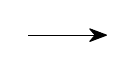
\begin{tikzpicture}[]\draw[->,>={Stealth[round,scale = 1.5]}](0,0)--(1,0) ;\end{tikzpicture}
  &
  \begin{tikzpicture}[baseline=(connection.base),connection/.style = {thick,circle,align = center}]\node(connection)[draw,connection]{连接};\end{tikzpicture}
  &
  \begin{tikzpicture}[baseline=(annotation.base),
    node distance = 5mm and 5mm,thick,
    nrb/.style={
      rectangle,draw=none,align=center,
      append after command={
        \pgfextra{
          \draw
          (\tikzlastnode.south east) --
          (\tikzlastnode.south west) --
          (\tikzlastnode.north west) --
          (\tikzlastnode.north east);
          \draw [-,dotted] (0,0)--(annotation.west);
        }
      }
    }
  ]
  \node at (1,0) (annotation)[nrb]{注释};
  \end{tikzpicture}
  \\
  \hline
\end{tabular}

\item 基本结构:
\begin{itemize}
  \item 顺序结构:
  \begin{figure}[H]
    \centering
    \begin{tikzpicture}[
      thick,node distance = 5mm and 5mm,
      startstop/.style = {rectangle,rounded corners,text centered},
      process/.style = {rectangle,text centered},
      io/.style = {trapezium,trapezium left angle = 70,trapezium right angle = 110,text centered},
      arrow/.style = {->,>=stealth}
    ]
      \node (start)[draw,startstop]{开始};
      \node (input)[draw,io,below = of start]{输入半径$R$};
      \node (process1)[draw,process,below = of input]{令$S=\pi\times R^2$};
      \node (process2)[draw,process,below = of process1]{令$L=2\pi\times R$};
      \node (output)[draw,io,below = of process2]{输出周长$L$,面积$S$};
      \node (stop)[draw,startstop,below = of output]{结束};
      \draw [->,>=stealth] (start.south) -- (input.north);
      \draw [->,>=stealth] (input.south) -- (process1.north);
      \draw [->,>=stealth] (process1.south) -- (process2.north);
      \draw [->,>=stealth] (process2.south) -- (output.north);
      \draw [->,>=stealth] (output.south) -- (stop.north);
    \end{tikzpicture}
    \caption{输入圆的半径R,输出圆的周长和面积}
  \end{figure}
  \item 循环结构:
  \begin{figure}[H]
    \centering
    \begin{tikzpicture}[
      thick,node distance = 5mm and 5mm,
      startstop/.style = {rectangle,rounded corners,text centered},
      process/.style = {rectangle,text centered},
      io/.style = {trapezium,trapezium left angle = 70,trapezium right angle = 110,text centered},
      arrow/.style = {->,>=stealth},
      decision/.style = {diamond,aspect = 2,inner sep = 0,text centered}
    ]
      \node (start)[draw,startstop]{开始};
      \node (input)[draw,io,below = of start]{输入半径$R$};
      \node (decision)[draw,decision,below = of input] {判断$R\geq 0$};
      \node (process1)[draw,process,below = of decision]{令$S=R$};
      \node (process2)[draw,process,right = of process1]{令$S=-R$};
      \node (output)[draw,io,below = of process1]{输出$S$};
      \node (stop)[draw,startstop,below = of output]{结束};

      \path (start.south) edge[->,>=stealth] (input.north);
      \path (input.south) edge[->,>=stealth] (decision.north);
      \draw [thick,->,>=stealth] (decision.east) -| (process2.north) node[midway,right]{\tiny 否};
      \path (decision.south) edge[->,>=stealth] node[midway,right]{\tiny 是} (process1.north);
      \path (process1.south) edge[->,>=stealth] (output.north);
      \draw [-] (process2.south) |- ($(process1.south)!0.5!(output.north)$);
      \path (output.south) edge[->,>=stealth] (stop.north);
    \end{tikzpicture}
    \caption{输入任意常数R,输出R的绝对值S}
  \end{figure}
  \item 选择结构:
  \begin{figure}[H]
    \centering
    \begin{tikzpicture}[
      thick,node distance = 5mm and 5mm,
      startstop/.style = {rectangle,rounded corners,text centered},
      process/.style = {rectangle,text centered},
      io/.style = {trapezium,trapezium left angle = 70,trapezium right angle = 110,text centered},
      arrow/.style = {->,>=stealth},
      decision/.style = {diamond,aspect = 2,inner sep = 0,text centered}
      ]
      \node (start)[draw,startstop]{开始};
      \node (input)[draw,io,below = of start]{输入$K$};
      \node (definition1)[draw,process,below = of input]{令$I=0$};
      \node (definition2)[draw,process,below = of definition1]{令$T=1$};
      \node (decision)[draw,decision,below = of definition2] {判断$I\leq K$};
      \node (process1)[draw,process,below = of decision]{令$T=T+I$};
      \node (process2)[draw,process,below = of process1]{令$I=I+1$};
      \node (output)[draw,io,below = of process2]{输出$T$};
      \node (stop)[draw,startstop,below = of output]{结束};

      \path (start.south) edge[->,>=stealth] (input.north);
      \path (input.south) edge[->,>=stealth] (definition1.north);
      \path (definition1.south) edge[->,>=stealth] (definition2.north);
      \path (definition2.south) edge[->,>=stealth] (decision.north);
      \path (decision.south) edge[->,>=stealth] node[midway,right]{\tiny 是} (process1.north);
      \path (process1.south) edge[thick,->,>=stealth] (process2.north);
      \draw [-] (process2.south) -- ($(process2.south)!0.3!(output.north)$) --++(-2,0) |- ($(definition2.south)!0.5!(decision.north)$);
      \draw [->,>=stealth] (decision.east) --++(.5,0) |- node[midway,right]{\tiny 否} ($(process2.south)!0.7!(output.north)$) -- (output.north);
      \path (output.south) edge[thick,->,>=stealth] (stop.north);
    \end{tikzpicture}
    \caption{输入任意自然数K,输出自然数1到K的和}
  \end{figure}
\end{itemize}     

\item 常见算法:

\begin{center}
  \begin{tabular}{cccc}
    求和算法 & 绘图算法 & 排序算法 & 穷举算法 \\
  \end{tabular}
\end{center}
\end{itemize}
\section{并行计算机体系结构}
\subsection{并行计算}
\begin{description}
\item[并行计算] 同时使用多台计算机或多处理器同时工作以提高计算速度和处理能力的计算方式。
\item[特点] 软件算法复杂、硬件结构复杂(多核微处理器)
\end{description}
\subsection{摩尔定律}
\noindent 微处理器的处理能力每\textbf{18个月到24个月}将增加一倍

\chapter{符号智能}
\section{搜索与问题求解}
\begin{description}
  \item[搜索] 人工智能技术中进行问题求解的基本技术
  \item[状态空间] 对智能体和环境当前情形的描述
  \item[动作] 智能体在某一状态下可执行的操作
  \item[问题的解] 初始状态到目标状态的一组行动序列
  \item[路径/代价] 一个完整的状态序列
  \item[最优解] 代价最小的解
\end{description}

\section{状态空间表示法}

\begin{description}
  \item[状态] 一组数据:$S_k=\left\{S_{k0},S_{k1},\dots\right\} $
  \item[操作(算符)] 
  \item[状态空间] 四元组:$(S,O,S_0,G)$ 
\end{description}
其中,  
\begin{itemize}
  \item $S$为\textbf{状态}集合
  \item $O$为\textbf{操作}集合
  \item $S_0$为\textbf{初始状态}
  \item $G$为若干具体状态或满足某些性质的\textbf{路径}信息
\end{itemize}
\section{盲目图搜索策略}

\begin{tabular}{l|l}
  \hline
  \textbf{广度优先搜索}(BFS) & \textbf{深度优先搜索}(DFS) \\
  \hline
  优先选择\textbf{最浅}节点扩展 & 优先选择\textbf{最深}节点扩展 \\
  \textbf{逐层}扩展 & \textbf{盲目}搜索 \\
  \textbf{高价}搜索 & \textbf{低价}搜索 \\
  有解问题能求最优解 & 有解问题不一定能求解 \\
  \hline
\end{tabular}

\section{启发式搜索}
\noindent 运用条件:
\begin{itemize}
  \item 问题没有明确的解
  \item 状态空间特别大
\end{itemize}

\noindent 估价函数$f(n)$:
\begin{equation*}
  f(n)=g(n)+h(n)
\end{equation*}
其中,$g(n)$为从初始状态$S_0$到节点$n$的\textbf{实际代价},启发函数$h(n)$为从节点$n$到目标状态$S_g$的最优路径的\textbf{估计代价}。

\begin{itemize}
  \item $h(n)$占比大时,趋向深度优先搜索
  \item $h(n)$占比小时,趋向广度优先搜索
\end{itemize}

在A算法中,若启发函数$h(n)<h^*(n)$,则称$h(n)$为\textbf{一致启发函数},此时A算法能得到最优解,称为\textbf{A*算法}。

如果启发函数h(n)满足以下条件:
\begin{equation*}
  h(n_i)-h(n_j)\leq C(n_i,n_j)\quad\text{且}\quad h(t) = 0
\end{equation*}

其中$n_j$是$n_i$的子节点,$t$是目标节点,$C(n_i,n_j)$是$n_j$与$n_i$间的\textbf{耗散值},

则称启发函数h(n)满足\textbf{单调限制条件}。

\section{知识表示}
人类知识符号化或模型化,转换为机器内部的一种数据结构

\begin{itemize}
  \item 一阶谓词逻辑表示法
  \item 产生式表示法
  \item 语义网络表示法
  \item 框架表示法
\end{itemize}


\section{一阶谓词逻辑表示法}
\begin{equation*}
  P(x_1,x_2,\dots,x_n)
\end{equation*}
其中,$P$为谓词,$x_1,x_2,\dots,x_n$为个体

\begin{itemize}
  \item 谓词连接词:
  \begin{tabular}{cccc}
    \hline
    否定 & 合取 & 析取 & 蕴涵 \\
    $\neg$ & $\land$ & $\lor$ & $\rightarrow$ \\
    \hline
  \end{tabular}
  \item 知识类别:
  \begin{description}
    \item[事实性知识] 合取、析取
    \item[规则性知识] 蕴涵
  \end{description}
  \item 特点
  \begin{itemize}
    \item 优点:
    \begin{description}
      \item[自然性] 与自然语言相近
      \item[精确性] 只取真假两种值
      \item[易实现] 便于计算机处理
      \item[严密性] 有严格的语法和语义规则
    \end{description}
    \item 缺点:
    \begin{description}
      \item[表达能力有限] 无法表示不确定性知识
      \item[推理能力有限] 无法进行复杂推理
      \item[知识表示有限] 难以表示启发性知识或元知识
    \end{description}
  \end{itemize}
\end{itemize}
\section{知识推理}
\begin{table}[H]
  \centering
  \begin{tabular}{lll}
    & 推理时所用的知识与证据 & 推出的结论 \\\hline\hline
    \textbf{确定性推理} & 确定 & 确定 \\\hline\hline
    \textbf{不确定性推理} & 不确定 & 不确定 \\\hline
    似然推理 && \\近似推理(模糊推理) && \\\hline
  \end{tabular}
\end{table}


\chapter{机器学习基础}
\section{机器学习的基本概念}
\noindent 机器学习:

通过算法解析数据、提取模式,并将这些模式转化为可用于预测或决策的模型

\noindent 机器学习类型:
\begin{description}
  \item[监督学习] 需要带标签的训练数据完成学习
  \begin{itemize}
    \item 分类
    \begin{itemize}
      \item K最近邻(KNN)
      \item 决策树
    \end{itemize}
    \item 回归
    \begin{itemize}
      \item 线性回归
      \item LASSO回归
    \end{itemize}
  \end{itemize}
  \item[无监督学习] 没有标签或正确答案的情况下,自己探索数据内在结构或关系
  \begin{itemize}
    \item 聚类
    \begin{itemize}
      \item K-means
      \item 均值漂移
    \end{itemize}
    \item 降维 
    \begin{itemize}
      \item PCA
      \item SVD
      \item t-SNE
      \item LLE
    \end{itemize}
  \end{itemize}
  \item[强化学习] 基于行为结果的奖励反馈调整策略
\end{description}

\section{回归}
\begin{itemize}
\item 回归:

预测数值

\item 多元线性回归的模型函数如下:
\begin{equation*}
y=\beta_0+\beta_1x_1+\beta_2x_2+\dots+\beta_nx_n+\epsilon 
\end{equation*}
其中:$y$是因变量,$x_1,x_2,\dots,x_n$是自
变量,$\beta_0$是截距项,$\beta_1,\beta_2,\dots \beta_n$ 是
各自变量的系数,$\epsilon$是误差项。

\item 梯度下降法:

迭代优化残差平方和(RSS)不断趋于最小
\begin{equation*}
  \text{RSS}(\beta_0,\beta_1)=\sum_{i=1}^{n}(y_i-\hat{y_i})^2=\sum_{i=1}^{n}(y_i-\beta_0-\beta_1x_i)^2
\end{equation*}
\end{itemize}
\section{分类}
\begin{itemize}
\item 分类:

将数据划分为不同类别

\item K最近邻(KNN)算法:

\begin{description}
  \item[数据准备] 数据清洗,数据处理,将每条数据整理成向量
  \item[计算距离] 计算待分类数据与训练集中每条数据的距离
  \item[选择K值] 选择距离最近的K个数据点
  \item[决策分类] 从K个数据点中选择出现频率最高的类别作为待分类数据的类别
\end{description}

不同K值分类准确率不同

\item 决策树:

做决策时层层递进的思考过程的监督学习模型
\end{itemize}
\section{降维}
\noindent 降维:简化模型、避免维度灾难

\noindent \textbf{主成分分析}(PCA):

通过线性变换将数据从高维空间映射到数据\textbf{方差最大}的低维空间

\begin{equation*}
  X_c = X - \bar{X}
\end{equation*}
$X$为数据矩阵,$\bar{x}$为平均数据,$X_c$为中心化后的数据矩阵
\begin{equation*}
  \lambda_i=\frac{1}{n-1}(X_cv_i)^T(X_cv_i)
\end{equation*}
\begin{equation*}
  \sum v_i=\lambda_iv_i
\end{equation*}
$\lambda_i$为$X$最大的特征值,则$v_i$为最大特征值对应的特征向量

\section{聚类}
\noindent 聚类:

将事物根据其特征分组成多个簇

\noindent \textbf{K均值算法}(K-means)步骤:

\begin{description}
  \item[选择K值] 确定要分成的簇的数量
  \item[初始化质心] 随机选择位置或数据点作为初始质心
  \item[分配数据点] 将每个数据点分配给距离最近的质心所属的簇
  \item[更新质心] 计算每个簇的质心,通常为所有数据点的均值
  \item[重复迭代] 重复步骤3和4,直到质心变化极小或达到预设的迭代次数
\end{description}

\section{强化学习}
\noindent 五个要素:
\begin{description}
  \item[环境] 智能体所处的外部世界
  \item[智能体] 强化学习中的核心部分,嵌入到环境中的决策实体
  \item[状态] 环境在某一时刻的具体情形
  \item[动作] 智能体在某一状态下可执行的操作
  \item[奖励] 智能体执行某一动作后从环境中获得的反馈信号
\end{description}

\begin{itemize}
  \item 基于价值函数的间接优化
  \item 基于策略梯度的直接优化
\end{itemize}

\noindent Q-learning算法:



\section{过拟合}
模型过于复杂,以至于很好地拟合了训练数据中的噪声和异常值,导致在新数据上的表现较差。

\chapter{神经网络与深度学习}
\section{人工神经网络}
\noindent 人工神经网络(ANNs):

模拟生物神经网络结构和功能的计算模型

\noindent 人工神经元:

大量人工神经元相互连接构成人工神经网络

\begin{equation*}
  y_i=f(\sum_{j=1}^{n}w_{ij}x_j-\theta_i)
\end{equation*}

其中,
\begin{description}
  \item[$\cdot\;x_i$] 输入
  \item[$\cdot\;w_i$] 权重
  \item[$\cdot\;\theta_i$] 偏置,微调神经元激活阈值
  \item[$\cdot\;f(\cdot)$] 激活函数,\textbf{引入非线性}
  \begin{description}
    \item[逻辑函数$\sigma$] $\sigma(z)=\frac{1}{1+e^{-z}}$
    \item[线性整流函数ReLU] $R(z)=\max(0,z)$
  \end{description}
  \item[$\cdot\;y_i$] 输出
\end{description}

\noindent 损失函数(Loss Function):对输出结果评分

\noindent 二分类交叉熵损失函数(Cross-Entropy) :
\begin{equation*}
  CE=-(y_i\log(\hat{y_i})+(1-y_i)\log(1-\hat{y_i}))
\end{equation*}

其中,
\begin{description}
  \item[$\cdot\;y_i$] 真实标签,取值为0或1,代表两个类别
  \item[$\cdot\;\hat{y_i}$] 模型预测的概率
\end{description}

\section{前馈神经网络}
\noindent 信息单向流动:输入层→隐藏层→输出层

\noindent 感知器(Perceptron):用于模式分类

\begin{tabular}{ccc}
  \hline
  感知器 & 非线性分类 & “异或”问题 \\
  \hline
  单层感知器 & 不能 & 不能 \\
  多层感知器 & 能 & 能 \\
  \hline
\end{tabular}

\noindent 卷积神经网络:一种前馈神经网络

\begin{description}
  \item[卷积层] 提取特征,生成特征图
  将卷积核在输入数据上滑动,并计算卷积核与输入数据的局部区域之间的点积
  
  RGB三个通道输出结果相加得到最终结果

  通过多通道多卷积核卷积层提取多种特征
  
  参数:
  
  \begin{description}
    \item[填充] 防止图像信息在卷积过程中缩小
    \item[步幅] 步幅增大,卷积层输出尺寸变小
  \end{description}
  \item[池化层] 简化提取的特征
  平均池化、最大池化
  \item[全连接层] 整合和转换特征,分类或回归预测
\end{description}

\section{反馈神经网络}
\noindent 信息循环传递

\noindent 循环神经网络(RNN):
\begin{description}
  \item[构成] 输入层、隐藏层、输出层
  \item[原理] 隐藏层状态由此刻的输入和上一刻的隐藏层状态同时决定
\end{description}

\noindent 长短期记忆神经网络(LSTM):
\begin{description}
  \item[引入记忆参数] 更好地保存长距离的序列依赖关系
  \item[引入遗忘门、输入门、输出门结构] 控制信息结构
\end{description}

\section{深度学习}
\begin{itemize}
  \item 基于人工神经网络的智能计算方法
  \item 机器学习的重要分支
  \item 核心基础算法:\textbf{卷积神经网络}、反向传播算法、梯度下降优化等关键技术
\end{itemize}

\noindent 计算机视觉领域的典型应用
\begin{itemize}
  \item 图像分类
  \begin{itemize}
  \item AlexNet:
  \begin{description}
    \item[神经网络层数更多]
    \item[ReLU作为激活函数] 运算简单
    \item[随机失活层(Dropout)] 增强模型泛化能力
  \end{description}
  \item ResNet:引入残差结构解决\textbf{退化问题}
  
  退化问题:更深的网络会伴随梯度消失、梯度爆炸等问题无法收敛,测试数据误差增大,训练数据误差增大
\end{itemize}
  \item 图像分割
  \begin{itemize}
    \item FCN
    \item Unet
  \end{itemize}
\end{itemize}


\chapter{生成式人工智能}
\section{生成式人工智能}
\begin{description}
  \item[应用场景] 生成文本、生成视频……
  \item[技术升级] 基于模板与规则→基于深度神经网络、融合专业场景
  \item[大模型] 
  \begin{tabular}{lll}
    \hline
    视觉 & 语言 & 多模态 \\
    感知 & 认知 & 内容创作 \\
    \hline
  \end{tabular}
  \item[AI Agent] 感知环境及需求、进行决策和执行动作的智能体
\end{description}

\section{对抗网络}
\noindent 使用两个网络互相竞争,称之为\textbf{对抗式}(adversarial)结构
\begin{itemize}
  \item 生成式对抗网络(GAN):

  能在非监督学习中生成新样本
  \item 深度卷积对抗式生成网络(DCGAN):
  \begin{itemize}
    \item 有监督学习的CNN与无监督学习的GAN的整合
    \item 通过编码运算控制人脸图像
  \end{itemize}
\end{itemize}

\section{Transformer模型}
\noindent 基于自注意力机制(Self-attention)的神经网络

\noindent 自注意力机制:
\begin{itemize}
  \item 优势:
  \begin{itemize}
    \item 更好建模\textbf{长距离}依赖关系
    \item 更好实现\textbf{并行计算}
  \end{itemize}
  \item 缺点:
  \begin{itemize}
    \item 不采用循环结构或卷积结构
  \end{itemize}
\end{itemize}

\noindent 位置向量:

明确单词位置关系,从而明确句子语义

多头注意力机制、缩放点积注意力机制

\noindent 解码器

N层*3个子层 = 3N
\begin{itemize}
  \item 掩码多头自注意力子层
  \item 编码-解码注意力子层
  \item 前馈网络子层
\end{itemize}
每个子层间采用残差连接(residual connection)和层归一化 (layer normalization)。

\noindent 编码-解码注意力子层:
\begin{itemize}
  \item 只对\textbf{隐层状态}做注意力计算
  \item 在解码过程中利用源语言信息
  \item 查询向量(q)来自\textbf{目标端}隐层状态
  \item 键向量(k)和值向量(v)来自\textbf{源端}隐层状态
\end{itemize}

\noindent Transformer应用:

自然语言处理、计算机视觉和语音识别以及\textbf{预训练语言模型}

\section{视觉处理系统}
\begin{itemize}
  \item 图像采集
  \begin{itemize}
    \item 纠正几何失真(图像坐标变换)
    \item 提高视觉质量(灰度映射、 直方图修正)
    \item 降低噪声干扰(空域滤波)
  \end{itemize}
  \item 特征工程:提取各种复杂度的特征(特征点检测)
  \item 模型训练
  \item 评价
\end{itemize}

\section{扩散模型}
\begin{itemize}
  \item 训练阶段
  \begin{enumerate}
    \item 向真实动作序列添加噪声
    \item 模型学习“如何还原原始动作”
  \end{enumerate}
  \item 生成阶段
  \begin{enumerate}
    \item 从纯噪声开始逐步迭代去噪
    \item 生成逼真的动作
  \end{enumerate}
\end{itemize}

\section{自然语言处理(NLP)}

研究能实现人与计算机之间用自然语言进行通信的各种理论和方法。

\noindent 阶段:

\begin{enumerate}
  \item 形式
  \item 语义
  \item 推理
  \item 语用 
\end{enumerate}

\section{大模型开发}
\begin{tabular}{llll}
  \hline
  预训练 & 通识教育 & 自监督学习 & 海量无标注数据 \\
  精调 & 专业教育 & & 任务相关少量数据 \\
  \hline
\end{tabular}

\section{AI Agent}
\begin{itemize}
\item AI Agent:

具有自适应性和智能性的软件实体,能代表用户或其它程序,以主动服务的方式完成一项工作。

Agent = LLM + 记忆 + 规划技能+ 工具使用
\item 多智能体:

一个松散耦合的Agent网络,通过交互、协作进行问题求解

\item 特点:

自主性、反应性、主动性、社会性

\item Agent技术架构:

感知记忆模块、规划决策模块、工具和行动模块
\end{itemize}

\chapter{行为智能与群智能}
\section{行为智能}
通过\textbf{观察环境},或通过\textbf{身体与环境的直接相互作用}产生的智能
\section{群智能}
群居昆虫的集体行为

\noindent 特点:

个体的行为很简单,\textbf{协同工作}时表现出非常复杂(智能)的行为特征

\noindent 蚁群算法:寻找最优路径
\begin{itemize}
  \item 要素:
  \begin{description}
    \item[信息素] 蚂蚁沿路径释放,随时间推移挥发
    \item[移动规则] 倾向于走信息素浓度高,路径短的路径
    \item[启发式信息] 距离、方向、障碍物等,有利于指导蚂蚁移动方向,提高搜索效率
  \end{description}
  \item 收敛性:蚁群算法具有较好的收敛性,能够在较短的时间内找到近似最优解
  \item 参数:信息素挥发速度、蚂蚁数量、移动概率
  \item 优化方法:遗传算法、粒子群算法等
  \item 步骤:
  \begin{enumerate}
    \item 初始化蚁群
    \begin{enumerate}
      \item 每只蚂蚁的方向和位置
      \item 信息素浓度
    \end{enumerate}
    \item 迭代搜索过程
    \begin{enumerate}
      \item 蚂蚁根据移动规则运动
      \item 更新路径信息素浓度
      \item 重复迭代过程
    \end{enumerate}
    \item 最优解输出
  \end{enumerate}
\end{itemize}

\section{具身智能}
基于物理身体进行感知和行动的智能系统
\par\noindent\textbf{虚拟环境}
\begin{description}
  \item[优势]安全、可扩展
  \item[要素]模拟器、资产、任务
  \item[模拟器] \phantom{}
  \begin{description}
    \item[物理仿真] 动力学的数学模型
    \item[感知信号渲染] 对机器人和周围环境的观测
    \item[要素] 渲染、物理特性、速度、对象类型和属性、动作建模、人机交互界面
  \end{description}
  \item[资产](静态/可交互):物体、场景、指令等数据结构
  \item[任务] \phantom{}
  \begin{itemize}
    \item 定位 Localization
    \item 视觉导航 Visual Navigation
    \item 对话驱动视觉导航 Visual Navigation
    \item 具身问答 Embodied Question Answering
  \end{itemize}
\end{description}
\par\noindent\textbf{Sim2Real迁移}:
\begin{enumerate}
  \item 环境
  \item 仿真
  \item 任务
\end{enumerate}

\section{进化计算}
\noindent 概念:
\begin{description}
  \item[进化计算] 模仿生物遗传并运用于复杂的优化问题
  \item[遗传算法] 基于进化过程中信息遗传机制和优胜劣汰自然选择原则的算法
  \item[基本遗传算法] (SGA)\marginpar{Simple Genetic Algorithm\hrule}
\end{description}

\noindent 要素:
\begin{description}
  \item[染色体编码] 将问题的解空间编码为染色体,用于遗传算法操作
  \item[适应度函数] 评估染色体好坏
  \item[遗传算子] \phantom{}
  \begin{description}
    \item[选择算子/复制算子] 挑选一部分父代个体进入子代
    \item[交叉算子/杂交算子] 挑选两个个体交换部分染色体形成新的个体
    \item[变异算子] 改变染色体基因的值
  \end{description}
  \item[参数] \phantom{}
  \begin{description}
    \item[N] 群体大小
    \item[T] 进化代数
    \item[Pc] 交叉概率(0.4-0.99)
    \item[Pm] 变异概率(0.0001-0.1)
  \end{description}
  \item[步骤] \phantom{}
  \begin{enumerate}
    \item 初始化群体:字符串编码、随机生成个体
    \item 迭代:计算个体适应值、通过三种算子(选择、杂交、变异)产生子代
    \item 计算最高适应值,输出最优值
  \end{enumerate}
\end{description}

\chapter{人工智能系统与应用}
\section{自动驾驶系统}
\begin{itemize}
  \item 分级
\begin{itemize}
  \item 环境感知系统
  \item 中央决策系统
  \item 底层执行系统
\end{itemize}
\end{itemize}





\appendix
\backmatter






\end{document}